%
\begin{figure}[htb!]
\begin{center}
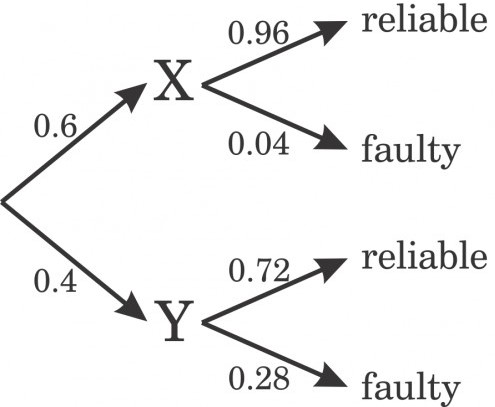
\includegraphics[width=0.5\textwidth]{A_4_1.png}
\end{center}
\end{figure}
Let Consider, Bernoulli random variables say $X,Y$ and $R$.
\begin{table}[h]
\resizebox{\columnwidth}{!}{
\begin{tabular}{|l|l|l|}
\hline
 & Refer to probability that product & Result \\ \hline
$Pr(X=1)$ & from supplier $X$ & $0.6$ \\ \hline
$Pr(Y=1)$ & from supplier $X$ & $0.4$ \\ \hline
$Pr(R=1)$ & is reliable &  \\ \hline
$Pr(R=0)$ & is faulty &  \\ \hline
$Pr(R=1/X=1)$ & from supplier $X$ is reliable & $0.96$ \\ \hline
$Pr(R=1/Y=1)$ & from supplier $Y$ is reliable & $0.72$ \\ \hline
\end{tabular}}
\caption{probability of random variables.}
\label{tab:my-table}
\end{table}
Required probability is $Pr(Y=1|R=1)$.So,
\begin{align}
&Pr(Y=1|R=1)=\frac{Pr(Y=1,R=1)}{Pr(R=1)}\\
&=\frac{Pr(Y=1)Pr(R=1/Y=1)}{Pr(X=1)Pr(R=1/X=1)+Pr(Y=1)P(R=1/Y=1)}\\
&=\frac{(0.4)(0.72)}{(0.6)(0.96)+(0.4)(0.72)}=0.334
\end{align}